\begin{withoutheadline}
\begin{frame}
\vspace*{-13mm}
\begin{figure}
	\hspace*{-4.2mm}
    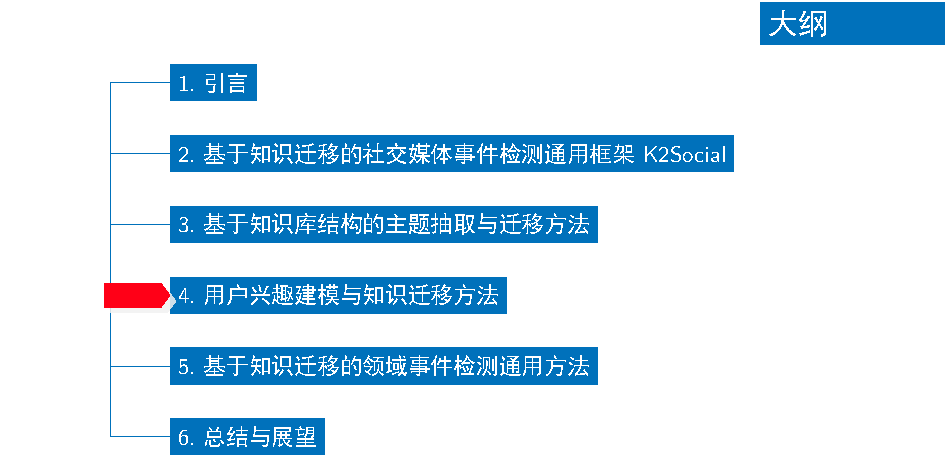
\includegraphics[width=1.0\paperwidth]{img/contents4_output.pdf}
\end{figure}

\end{frame}
\end{withoutheadline}

\section{用户兴趣建模与知识迁移方法}


%TODO 要说明对突发事件检测有迫切需求
\begin{frame}
\frametitle{Motivation}	
issue
说明对突发事件检测有迫切需求

\pdfnote{前面一节中已经分析了知识迁移对事件检测准确性的提升,这一小节中我们分析知识迁移对事件检测时效性的提升}
\end{frame}

\begin{frame}
\frametitle{突发事件的特点}
这里放一幅插图,说明突发事件的特点是不同兴趣的用户在同一时间窗口内都关心的事件。
\pdfnote{突发事件的特点是不同兴趣的用户在同一时间窗口内都关心的事件。}
\end{frame}


\begin{frame}
\frametitle{Motivation}
\begin{figure}[h]
		\setlength{\abovecaptionskip}{0.cm}
        \setlength{\belowcaptionskip}{0.cm}
        \centering
		\caption{社交媒体关注网络用于扩充个人自我描述信息示意图}
        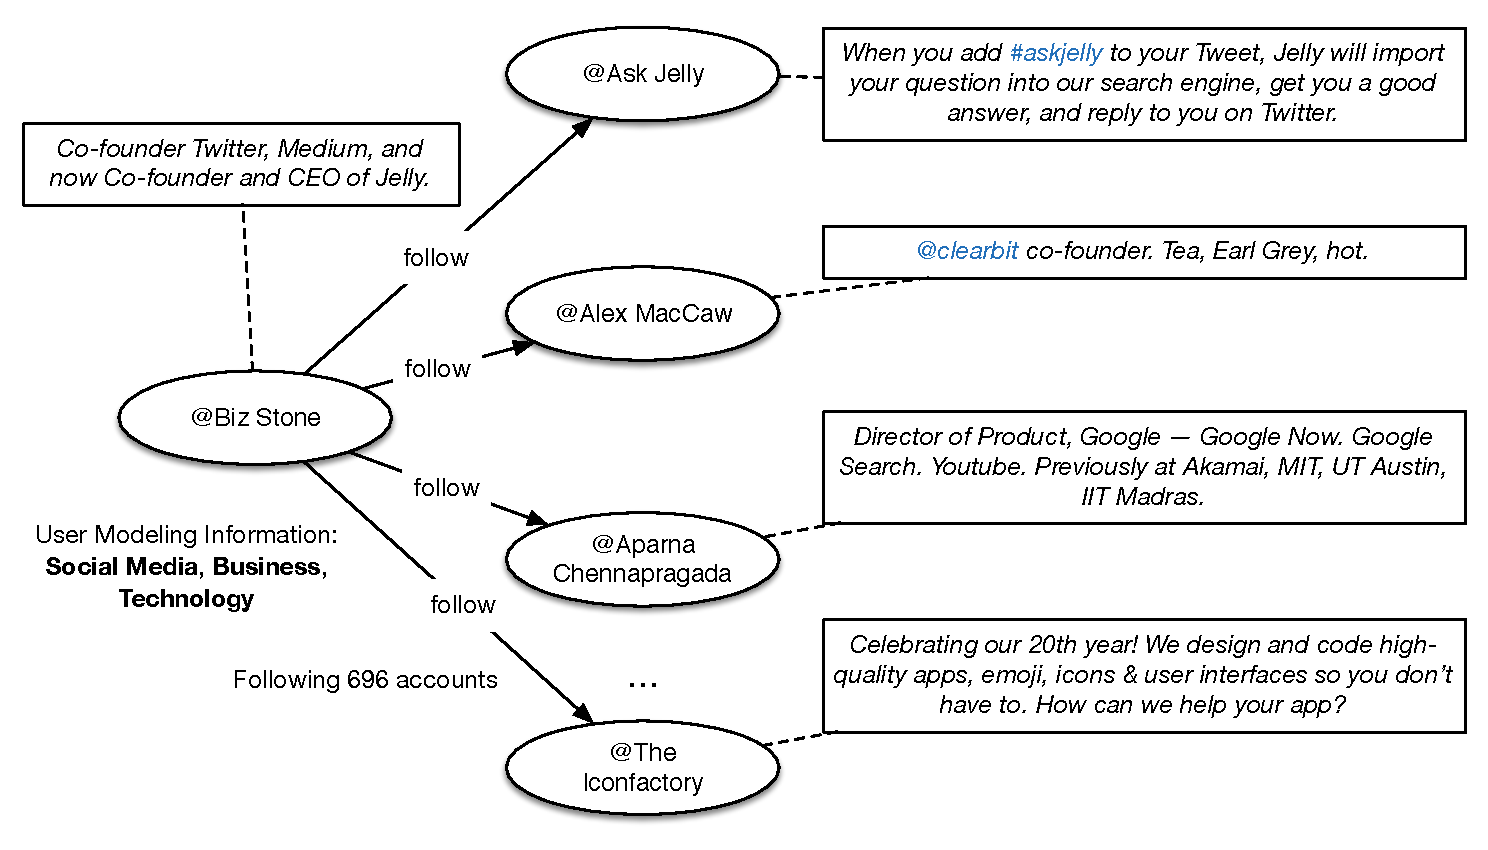
\includegraphics[width=0.9\columnwidth]{img/UMIETM/UMIETM_profile.pdf}
\end{figure}
\end{frame}

\begin{frame}
\frametitle{我们的方法}
UMIETM模型(User Modeling Based Interest and Event Topic Modeling)
\begin{itemize}
\item 使用用户个人描述信息与用户关注网络建模用户兴趣分布
\item 将用户兴趣知识迁移到微博中
\item 区分用户兴趣与突发事件
\end{itemize}

\vspace{-3mm}
\begin{figure}
	\setlength{\abovecaptionskip}{0.cm}
	\setlength{\belowcaptionskip}{0.cm}
	\caption{UMIETM概率模型}
	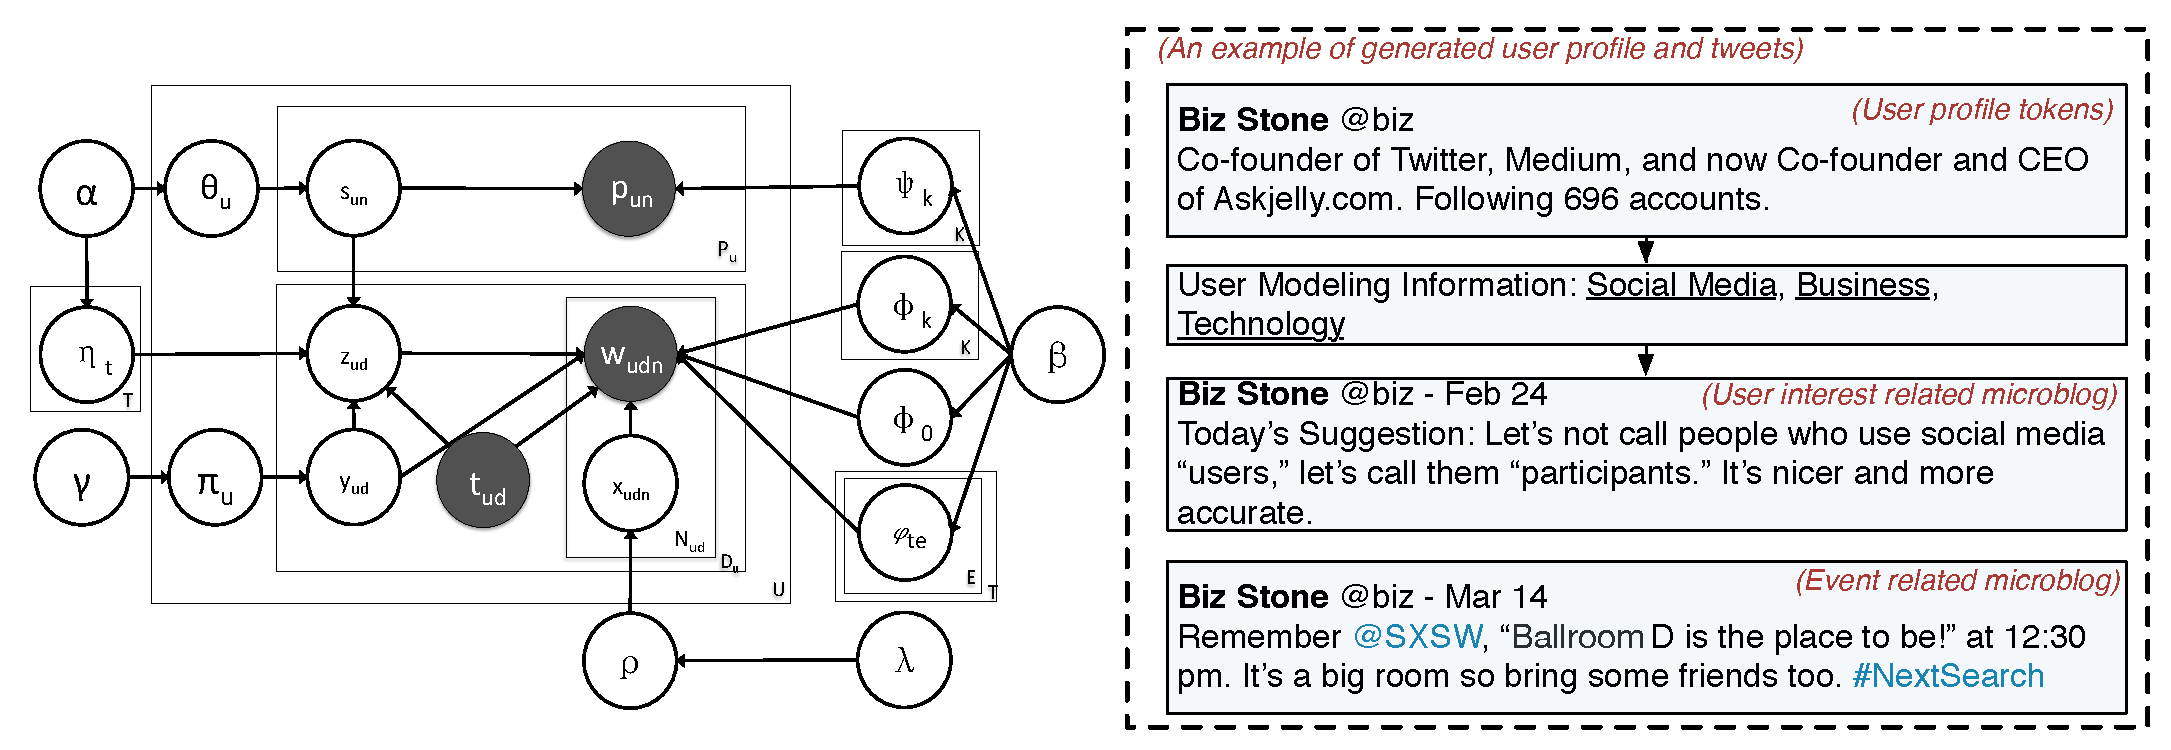
\includegraphics[width=1.0\textwidth]{img/UMIETM/model.pdf}
	\label{fig:modelUMIETM}
\end{figure}
\pdfnote{(左侧)UMIETM概率模型示意图。(右侧)示例用户Biz Stone的两类文本(用户兴趣相关的文本与突发事件相关的文本)的示意图。其个人简档揭示出其个人兴趣主要集中在社交网络、商业、科技领域。依据UMIETM模型,可以检测出他2016年2月24日发布的有关社交网络中用户角色定位的文本可以被检测为与个人兴趣相关;2016年3月14日发布的有关SXSW的文本则与个人兴趣都不相关,结合该时间窗口内更多的其他文本,可以将判断这条文本和突发事件相关,事实上SXSW是一个在3月11日到20日之间举行的盛大音乐节。}
\end{frame}


\begin{frame}
\frametitle{UMIETM知识迁移算法}

\begin{columns}[t]
\column{0.38\paperwidth}
计算用户兴趣分布:
\begin{equation}
\scriptsize
\label{timeUserTagLDAIVsamplingForS}
\begin{aligned}
&p(s_{un}=k|s_{\neg{un}},\vec{p},\alpha,\beta)\\
&\propto \frac{c^{(p)}_{uk}+\alpha}{c^{(p)}_{u,.}+K\alpha}
\frac{c^{(p)}_{kv}+\beta}{c^{(p)}_{k,.}+V\beta}\\
\end{aligned}
\end{equation}

\column{0.46\paperwidth}
\scalebox{0.65}{
\begin{minipage}{.7\paperwidth}
\begin{algorithm}[H]
\begin{spacing}{0.8}
	%\scriptsize
    \caption{UMIETM知识迁移算法} %title
    \label{alg:UMIETM_batch} %label
    \DontPrintSemicolon
    initiate the topic label and the statistics \\
    \For {\(i=1:I_1\)}{
        \For{\(u\) in  user set \(\mathcal{U}\)}{
            \For{\(n\) = \(1:P_u\)}{
                sample profile's hidden topic \(s_{un}\) by (\ref{timeUserTagLDAIVsamplingForS})\, update \(s_{un}\), \(c^{(p)}_{u,k}\) and \(c^{(p)}_{k,v}\)
            }%end of n
        }%end of u
    }%end of i
    \For{iteration \(i=1:I_2\)}{
        \For{\(t=1:T\)}{
            \For{\(u\) in  user set \(U_t\)}{
                \For{\(d\) = \(1: D_u\) }{
                    sample \(y_{ud}\) and \(z_{ud}\) by (\ref{timeUserTagLDAIVJointSamplingForY0Z}), (\ref{timeUserTagLDAIVJointSamplingForY1Z})\\
                    \If{\(y_{ud}=0\)}{
                        update \(z_{ud}\), \(y_{ud}\), \(c^{(0)}_u\), \(c^{(0)}_{u,k}\), \(c^{(0)}_{k,v}\)
                    }\Else{
                        update \(z_{ud}\), \(y_{ud}\), \(c^{(1)}_u\), \(c^{(1)}_{t,e}\), \(c^{(1)}_{t,e,v}\)
                    }
                    \For{\(n\) in \(1,\cdots,N_{ud}\)}{
                        sample \(x_{udn}\) by (\ref{timeUserTagLDAIVsamplingX0}), (\ref{timeUserTagLDAIVsamplingX1})\\
                        \If{\(x_{udn}=0\)}{
                            update \(x_{udn}\), \(M^{\rho}_0\), \(c^{(B)}_v\)
                        }\Else{
                            update \(x_{udn}\), \(M^{\rho}_1\), \(c^{(0)}_{k,v}\), \(c^{(1)}_{t,e,v}\)
                        }
                    }%end of n
                }%end of d
            }%end of u
        }%end of t
    }%end of i
\end{spacing}
\end{algorithm}
\end{minipage}
}
\end{columns}
\pdfnote{两阶段进行吉布斯采样}
\end{frame}

